An Alloy model is provided to present a formal description of the system. 
The goals of this kind of analysis are to check the consistency of the model and to find possible errors and corner cases in the requirements.\\
A formal model is also useful to express complex facts which are not captured by the domain class diagram such as the constraints involving subcriptions, scores, timestamps, battle and tournament states.\\ \\

\subsection{Model Code}
\begin{lstlisting}[language=alloy]
open util/integer

//SIGNATURES

sig Email {}

sig Password {}

sig GithubUsername {}

abstract sig User {

    email: Email,

    password: Password

}

sig Student extends User {

    username: one GithubUsername

}

sig Educator extends User {

    createsTournament: set Tournament,

    createBattle: set Battle

}






sig Timestamp {

    time: Int

} { 
    time >= 0 
}

one sig SystemTimestamp {

    ts: Timestamp

}

pred earlierThan [t1, t2: Timestamp] {

    int t1.time < int t2.time

}

pred earlierEqual [t1, t2: Timestamp] {

    int t1.time <= int t2.time

}

enum TournamentState { Subscription, Ongoing, Ended }

sig Tournament {

    subscriptionDeadline: Timestamp,

    state: TournamentState ,

    isManaged: some Educator,

    battles: set Battle,

    participants: set Student -> one Score

}

sig TestCase {}

sig CodeKata {

testCases: some TestCase

}

enum Bool { True, False }

enum ProgrammingLanguage { Python, Java, C }

enum BattleState { TeamFormation, SubmissionPhase, ConsolidationPhase, Finished }

sig Battle {

    state: BattleState ,

    participants: set Team,

    registrationDeadline: Timestamp,

    submissionDeadline: Timestamp,

    minTeamSize: Int,

    maxTeamSize: Int,

    programmingLanguage: ProgrammingLanguage,

    codeKata: CodeKata,

    a1Eval: Bool,

    a2Eval: Bool,

    a3Eval: Bool,

    manualEval: Bool

}  {

    earlierThan[registrationDeadline,submissionDeadline]

    minTeamSize > 0

    maxTeamSize >= minTeamSize

}

sig Score {

    value: Int

} {

    int value >= 0

}

sig Submission {

    ts: one Timestamp,

    functionalScore: one Score,

    timelinessScore: one Score,

    a1Score: lone Score,

    a2Score: lone Score,

    a3Score: lone Score,

    qualityScore: one Score,

    manualScore: lone Score,

    overallScore: one Score,

    battle: Battle

}

sig ApiToken{}

sig InviteCode{}

sig Team {

    submissions: set Submission,

    participates: one Battle,

    members: some Student,

    battleScore: one Score,

    apiToken: one ApiToken,

    inviteCode: one InviteCode

}


//INTEGRITY CONSTRAINTS

// each password is associated to some user ( some registration may have the same password )
fact eachPasswordToSomeUser{
all p : Password | ( some u : User | u. password = p)
}

// each Int associated to at most 1 timestamp
fact oneTimestampPerInteger{
all i:Int | ( lone t : Timestamp | t.time = i)
}

// each Intt associated to at most 1 score
fact oneTimestampPerInteger{
all i:Int | ( lone s : Score | s.value = i)
}

// each username is associated to a unique student
fact eachGitHubUsernameToOneStudent{
all u : GithubUsername | ( one s : Student | s. username = u)
}

// each ApiToken is associated to a unique team
fact eachApitTokenToOneTeam{
all a : ApiToken | ( one t : Team | t. apiToken= a)
}

// each InviteCode is associated to a unique team
fact eachInviteCodeToOneTeam{
all i : InviteCode | ( one t : Team | t. inviteCode= i)
}

// each email is associated to a unique user 
fact eachEmailToOneUser{
all e : Email| ( one u : User | u. email= e)
}

// each tournament has 1 creator
fact eachTournamentHasOneCreator{
all t : Tournament | ( one e : Educator | t in e.createsTournament )
}

// each battle has 1 creator
fact eachBattleHasOneCreator{
all b : Battle | ( one e : Educator | b in e.createBattle)
}

// each battle belongs to only a tournament
fact eachBattleToOneTournament{
all b: Battle| (one t : Tournament | b in t.battles )
}

// each testcase belongs to only a code kata
fact eachTestCaseToOneCodeKata{
all t: TestCase| (one c : CodeKata| t in c.testCases )
}

// each CodeKata belongs to only a battle
fact eachCodeKataToOneBattle{
all c: CodeKata| (one b : Battle| c in b.codeKata )
}

// each Submission belongs to only a Team
fact eachSubmissionToOneTeam{
all s: Submission| (one t : Team| s in t.submissions )
}

// coherence between battle's participants and team's participates
fact coherenceBetweenParticipantsAndParticipate{
all t: Team, b: Battle | t in b.participants <==> t.participates = b
}








//ADDITIONAL CONSTRAINTS

//tournament is on ongoing state if and only if subscription deadline has elapsed
fact tournamentStateCoherentWithSystemTimestamp{
all t:Tournament | earlierThan[t.subscriptionDeadline, SystemTimestamp.ts] <=> t.state = Ongoing
}

// battle states coherent with system timestamp
fact battleStateCoherentWithSystemTimestamp{
all b:Battle | 
    (earlierThan[SystemTimestamp.ts, b.registrationDeadline] 
        implies b.state = TeamFormation) and
    ((earlierEqual[ b.registrationDeadline,SystemTimestamp.ts] and earlierThan[ SystemTimestamp.ts, b.submissionDeadline]) 
        implies b.state = SubmissionPhase) and
    (earlierEqual[ b.submissionDeadline,SystemTimestamp.ts] 
        implies (b.state = ConsolidationPhase or b.state = Finished) )
}

//submission ts come before system timestamp
fact submissionTsBeforeSystemTimestamp{
all s:Submission | earlierEqual[s.ts, SystemTimestamp.ts]
}

// each student can subscribe only once to a tournament
fact eachStudentSubscribesMostOnce{
all t:Tournament, s:Student | #t.participants[s] <= 1
}

// tournament creator is also managing the tournament (tournament has at least 1 educator managing it)
fact creatorCanManage{ 
all e: Educator, t:e.createsTournament  | e in t.isManaged 
}

// tournament's participants scores are the sum of battle scores obtained by the teams the student is a member of in the battles of that tournament
fun allStudentTeamsInEndedBattles[s:Student]:set Team{
{t:Team | s in t.members and t.participates.state = Finished}
}
fun totalTournamentScore[t: Tournament, s: Student]: Int {
sum te: t.battles.participants&allStudentTeamsInEndedBattles[s] | int te.battleScore.value
}
fact TournamentParticipantsScoreComputation{ 
all t: Tournament, s: Student | #t.participants[s] = 1 implies int t.participants[s].value = int totalTournamentScore[t,s]
}

// submission's quality score is the sum of all aspects scores
fun add3Scores[a, b, c: Score]: Score {
{i: Score | int i.value = integer/add[ integer/add[a.value, b.value], c.value]}
}
fact qualityScoreCombinesAspectsScores {
all s:Submission | s.qualityScore = add3Scores[s.a1Score, s.a2Score, s.a3Score] 
}

// submission's overall score is the sum of all the scores
fun add4Scores[a, b, c, d: Score]: Score {
{i: Score | int i.value = integer/add[integer/add[integer/add[a.value,b.value],c.value], d.value]}
}
fact OverallScoreCombinesAutoAndManualScore {
all s:Submission | s.overallScore = add4Scores[s.functionalScore, s.timelinessScore, s.qualityScore, s.manualScore]
}

// battleScore is the overall score of the team's last submission
fun lastSubmission[t: Team]: one Submission {
{ s: t.submissions | no su: t.submissions - s | earlierThan[s.ts,su.ts] }
}
fact battleScoreIsLastOverallScore {
all t: Team | (#t.submissions= 0 implies int t.battleScore.value = 0) and
	      (#t.submissions >0 implies int t.battleScore.value = int lastSubmission[t].overallScore.value)
}

// battle registration deadline comes after tournament subscription deadline
fact RegistrationAfterSubscription {
all b:Battle,to:Tournament | b in to.battles implies earlierThan[to.subscriptionDeadline,b.registrationDeadline]
}

// Student participates only to battles that belong to tournaments he is enrolled in
fact OnlyBattlesInEnrolledTournament {
all s:Student, te:Team, to:Tournament | (s in te.members and te.participates in to.battles) implies (#to.participants[s] = 1)
}

// a battle can be associated to a tournament only if the tournament is not in registration phase anymore
fact NoBattleInTournamentSubscription {
no t:Tournament | t.state = Subscription and #t.battles > 0
}

// if a tournament is ended, then all its battles must be ended too
fact AllBattleEndedIfTournamentEnded {
all t:Tournament| t.state = Ended implies (all b: t.battles | b.state = Finished)
}

// if a battle is in teamFormation/submission/consolidation state, then its tournament must be on ongoing state
fact TournamentOngoingIfBattleNotEnded {
all t:Tournament, b:t.battles | b.state != Finished implies (t.state != Ended)
}

// automated scores of the submission are present only if they are enabled in the battle
fact AutomatedScorePresentIfEnabled {
all s:Submission | (#s.a1Score = 1 <==> s.battle.a1Eval = True) and
		   (#s.a2Score = 1 <==> s.battle.a2Eval = True) and
		   (#s.a3Score = 1 <==> s.battle.a3Eval = True) 
}

// a submission can be associated to a battle only if the battle is in the submission/consolidation/ended state 
fact noSubmissionInTeamFormationPhase {
no s:Submission | s.battle.state = TeamFormation
}

// a submission can happen only after the registration deadline and before the battle's submission deadline
fact SubmissionInSubmissionPhase {
all s:Submission | earlierThan[s.battle.registrationDeadline,s.ts] and earlierThan[s.ts,s.battle.submissionDeadline]
}

// a submission to a battle can occur only if the team is participating to the battle
fact TeamSubmitsOnlyToCorrectBattle {
all t:Team, s:Submission | (s in t.submissions) implies (s.battle = t.participates)
}

// a battle can be created only by educators managing the tournament the battle belongs to
fact BattleCreatedByManager {
all b:Battle, e:Educator, t:Tournament | (b in e.createBattle and b in t.battles) implies (e in t.isManaged)
}

// team members count respects battle's settings
fact TeamSize {
all t:Team | #t.members >= int t.participates.minTeamSize and
	     #t.members <= int t.participates.maxTeamSize
}

// a student can participate to a battle only with 1 team
fact OnlyOneTeamPerBattle {
no t1,t2:Team,s:Student  | t1 != t2 and
			   s in t1.members and
			   s in t2.members and
			   t1.participates = t2.participates
}

// tournament scores initialized to 0  (if tournament is not started yet or none of its battles are ended)
fact ZeroInitializedTournamentScores {
all s:Student, to:Tournament, b:Battle | (#to.participants[s] = 1 
	and (to.state = Subscription or (b in to.battles and b.state != Finished) ) ) implies to.participants[s].value = 0
}

// if a submission comes after another, then its timeliness score should be lower
fact LowerTimelinessScore {
all b:Battle, disj s1,s2:Submission  |  (b in s1.battle and b in s2.battle and earlierThan[s1.ts,s2.ts]) 
    	implies 
    int s1.timelinessScore.value > int s2.timelinessScore.value
}

// There no exist 2 concurrent submissions from same team
fact NoConcurrentSubmission{
all t:Team| no disj s1,s2:t.submissions  |  s1.ts.time = s2.ts.time
}

// a student can be enrolled to a tournament at most once
fact NoDoubleEnrollment {
no to:Tournament, s:Student| #to.participants[s] > 1 
}

// a battle can enter ConsolidationPhase only if manual evaluation is enabled
fact consolidationPhaseOnlyWithManualEval{
all b: Battle | b.state = ConsolidationPhase implies b.manualEval = True
}

// manual score can be present only if the related battle is in consolidation phase or finished
fact ManualScoreOnlyInConsolidationOrFinished{
all s: Submission | #s.manualScore = 1 implies (s.battle.state = ConsolidationPhase or s.battle.state = Finished)
}

// manual score in the submission is present only if its enabled in the battle
fact ManualScorePresentIfEanbled {
all s:Submission | #s.manualScore = 1 implies s.battle.manualEval = True 
}

// manualScore can be present only in the last submission
fact manualScoreOnlyInLastSubmission{
all t: Team, s: t.submissions | #s.manualScore = 1 implies s = lastSubmission[t]
}

// if a battle is ended, manualScore must be present in the last submission
fact manualScoreWhenBattleFinished{
all t: Team | (t.participates.state = Finished and t.participates.manualEval = True) 
        implies 
    #lastSubmission[t].manualScore = 1
}






// Show predicates
pred world1{
#Tournament=1
#Educator=2
#Battle=2
#Tournament.isManaged=2
}

pred world2{
#Tournament=1
#Educator=1
#Battle=2
#Team=2
#Submission=3
}

run world1  for 6
\end{lstlisting}

\subsection{Static analysis}
\begin{lstlisting}[language=alloy]
//Check that all students enrolled in the tournament have 0 tournament score during subcription phase
assert StudentTournamentScoreBeforeStart{
    all t : Tournament, s:Student | (#t.participants[s]=1 and t.state=Subscription) implies int t.participants[s].value = 0
}
check StudentTournamentScoreBeforeStart for 4

//Check that all students enrolled to tournament without any finished battle have 0 tournament score
assert StudentTournamentScoreNoFinishedBattles{
    all t : Tournament, s:Student|(#t.participants[s]=1 and t.state=Ongoing and (no b: t.battles, te:b.participants |  b.state = Finished and s in te.members)) implies int t.participants[s].value = 0
}
check StudentTournamentScoreNoFinishedBattles for 4

//Check that all students enrolled to tournament with a tournament score greater than 0 have participated to at least 1 finished battle in that tournament
assert StudentParticipatesWithTeam{
    all t : Tournament, s:Student| int t.participants[s].value > 0 implies ( some b:t.battles,te:t.battles.participants | b.state=Finished and s in te.members)
}
check StudentParticipatesWithTeam for 4

//Check that all teams enrolled to the battle have 0 battle score before their first submission
assert TeamScoreZeroBeforeSubmissions{
    all b : Battle, te:b.participants | (#te.submissions = 0) implies int te.battleScore.value = 0
}
check TeamScoreZeroBeforeSubmissions for 4

//Check that all teams having battle score greater than 0 have at least 1 submission
assert TeamNonZeroScore{
    all b : Battle, te:b.participants |  int te.battleScore.value > 0  implies  (#te.submissions > 0)
}
check TeamNonZeroScore for 4

//Check that all teams's latest submission have been manually evaluated if a battle is ended
assert AllTeamsManuallyEvaluated{
    no b : Battle |  b.manualEval = True and b.state=Finished and (some te:b.participants | #lastSubmission[te].manualScore = 0)
}
check AllTeamsManuallyEvaluated for 4

\end{lstlisting}
\hfill \break
The alloy model previously presented focuses on the most important entities and attributes of the domain, which are strictly necessary to describe the main functionalities of the system. Indeed, some concepts such as time and scores have been simplified to be easily handled by the Alloy Analyzer and syntax.\\
Images of three world examples are shown below, the first focuses on educators, tournaments and battles, while the second and the third ones include all the aspects related to students, teams and submissions.
\newpage

\begin{figure}[H]
    \vspace{-2cm}
    \hspace{-4cm}
    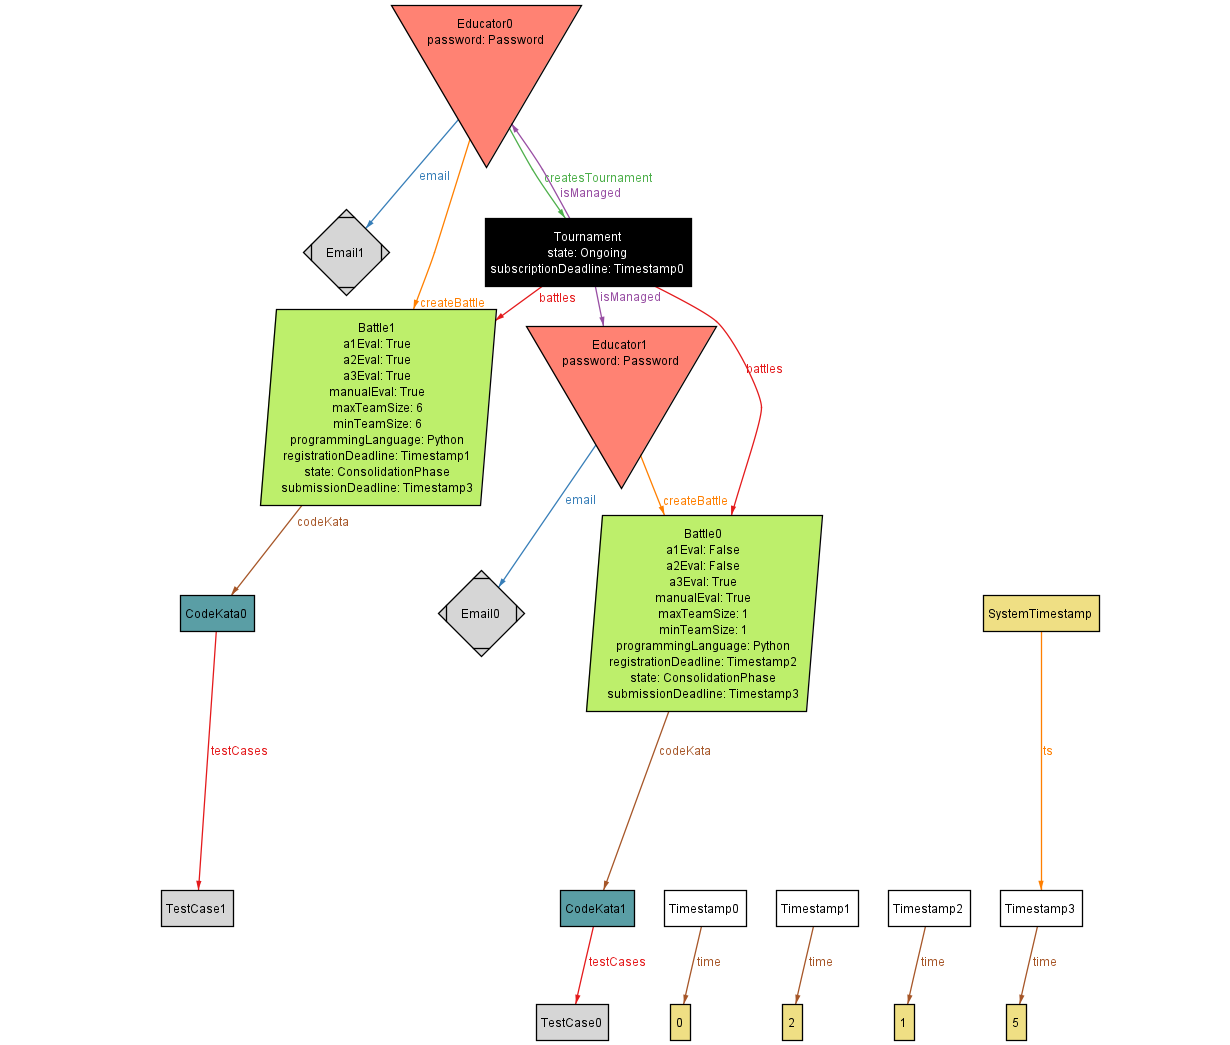
\includegraphics[width=1.65\textwidth]{Alloy/world1.png}
    \vspace{0.2cm}
    \caption{World1, generated with the \textit{world1} predicate}
\end{figure}
\newpage
\begin{figure}[H]
    \centering
    \vspace{-4cm}
    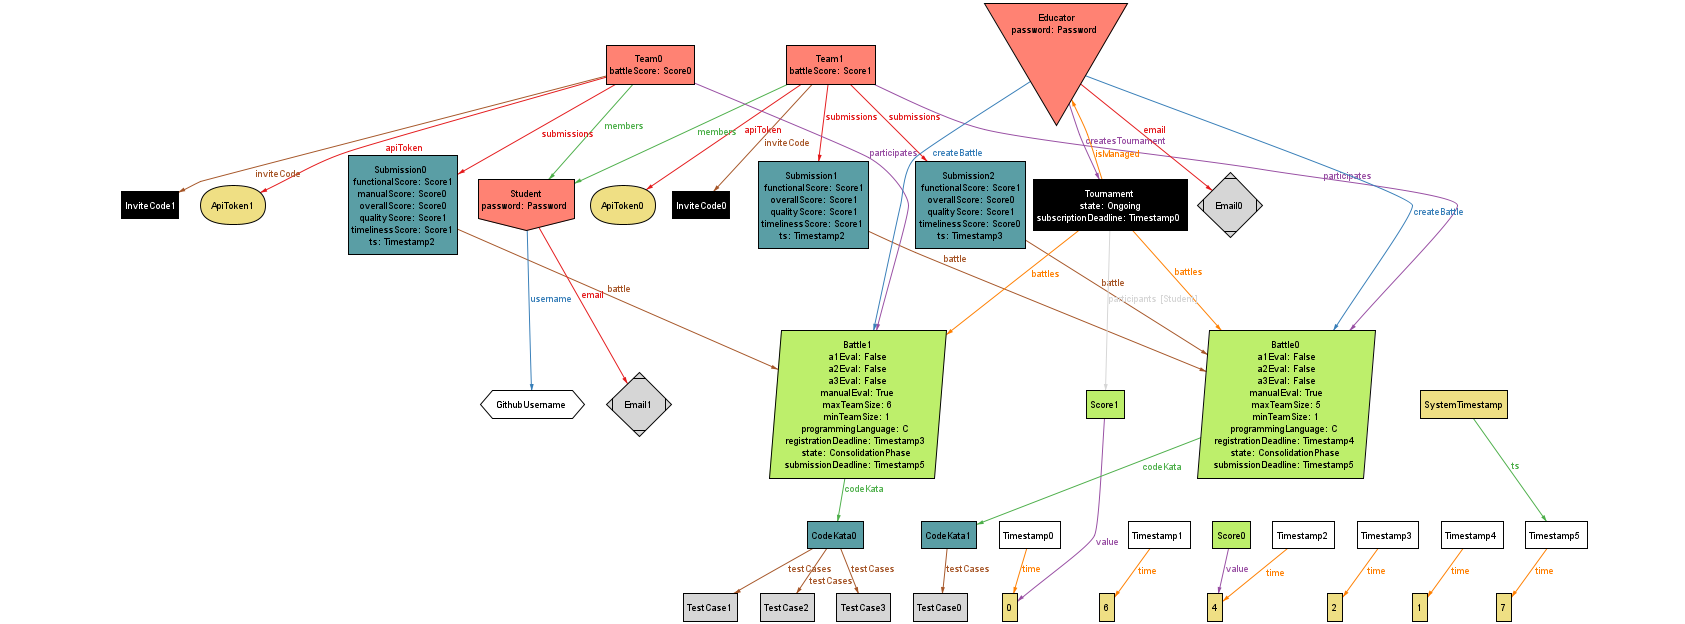
\includegraphics[width=1.65\textwidth,angle=90,origin=c]{Alloy/world2.png}
    \caption{World2, generated with the \textit{world2} predicate}
\end{figure}
\newpage
\begin{figure}[H]
    \centering
    \vspace{-4cm}
    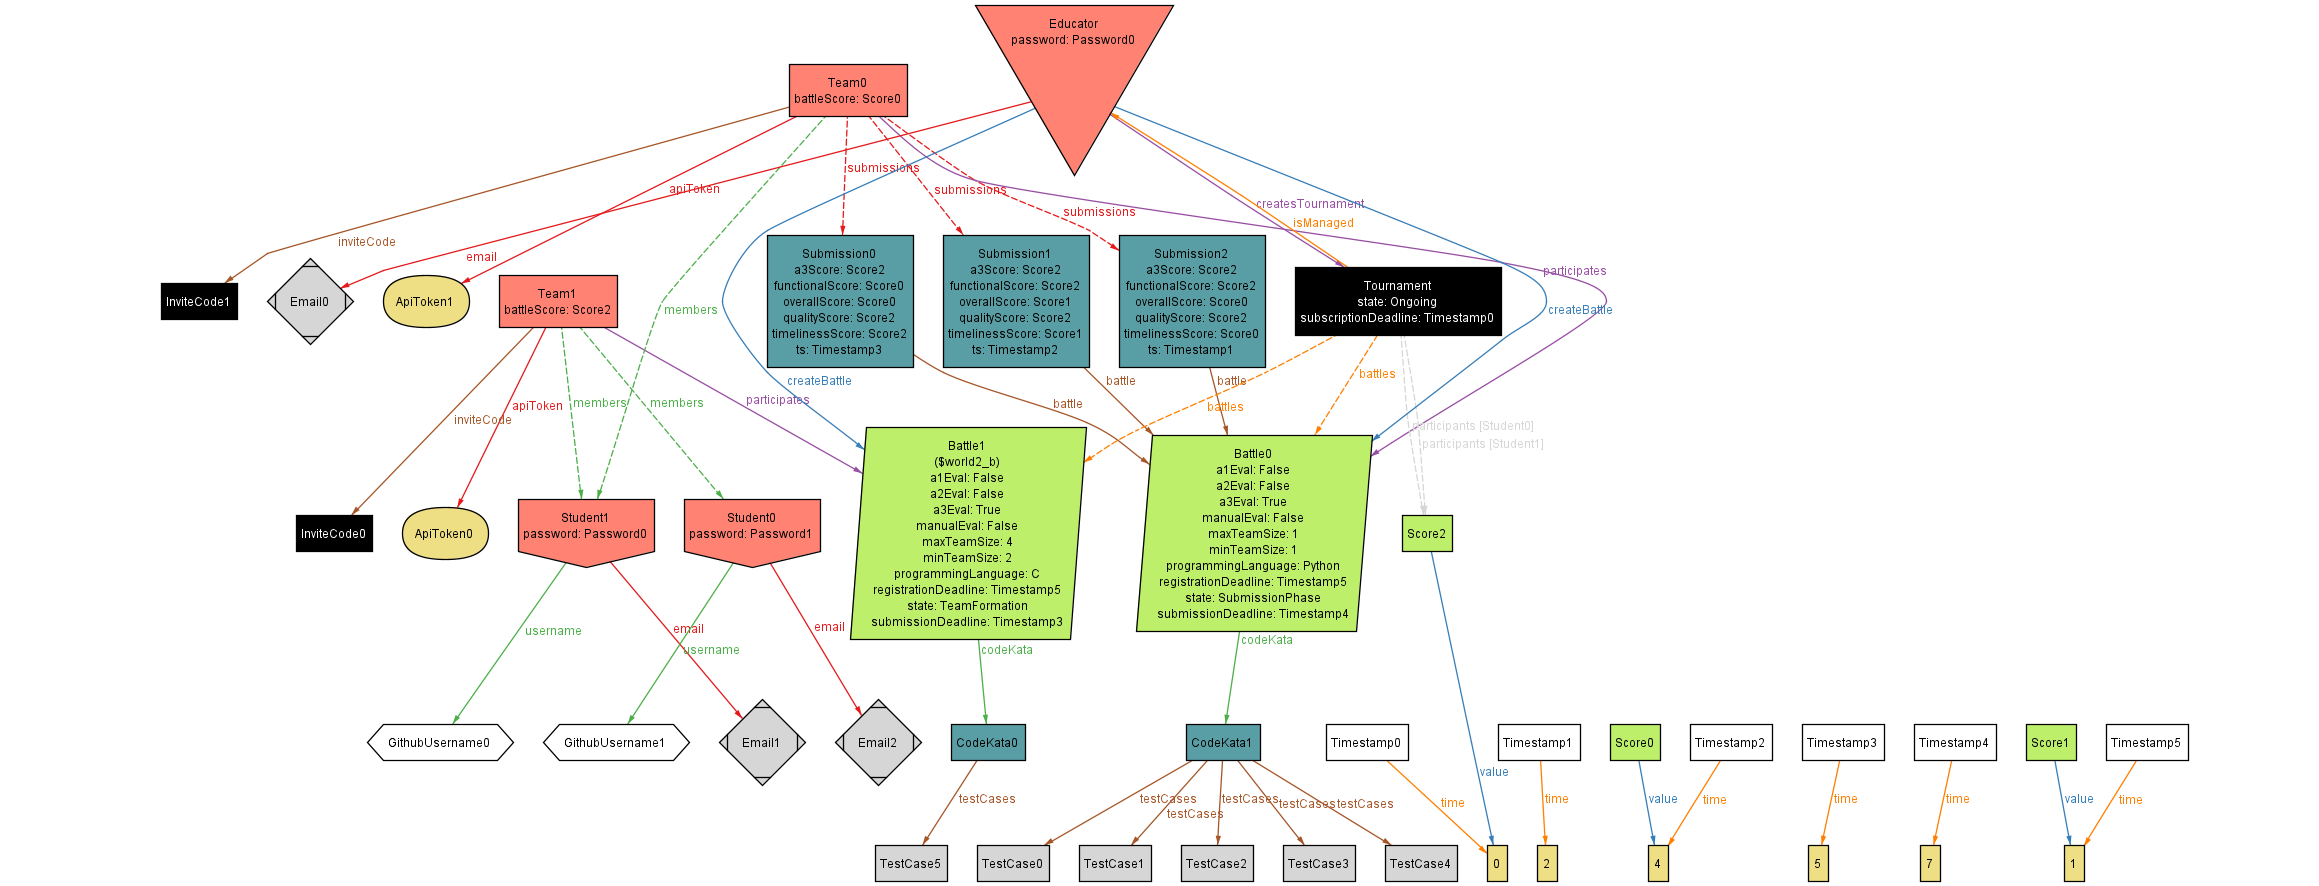
\includegraphics[width=1.65\textwidth,angle=90,origin=c]{Alloy/world3.png}
    \caption{World2, generated with the \textit{world2} predicate}
\end{figure}
\newpage